\section{Registrasie}
\subsection{Gebruikersgeval}

\begin{figure}[htbp]
    \centering
    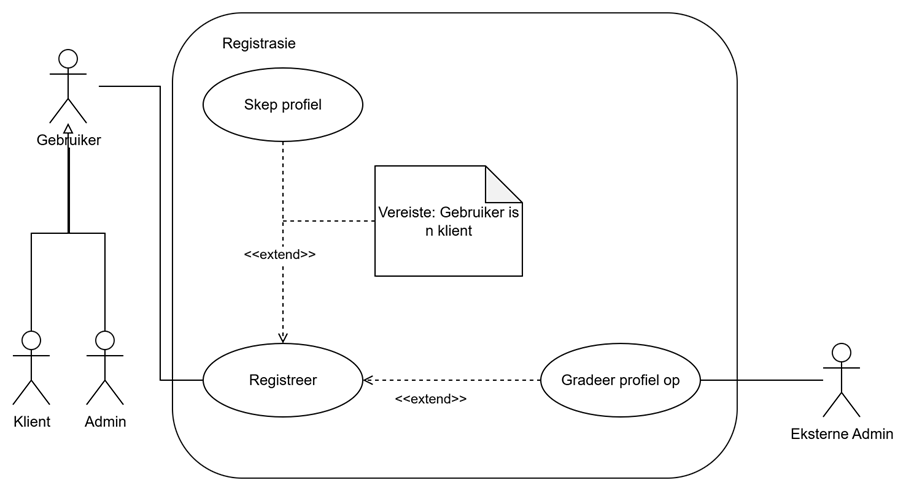
\includegraphics[width=\textwidth]{figures/usecase/registration.png}
    \caption{Gebruikersgeval vir Registrasie}
    \label{fig:registrasie_use_case}
\end{figure}

Volgens funksionele vereiste FREQ-USR-001 moet gebruikers kan registreer met hul naam en van, e-pos adres. Die registrasie proses begin op die registrasie skerm (\autoref{fig:registration_screen}). Verder volgens FREQ-USR-002 moet gebruikers wie 'n bestelling wil plaas 'n profiel skep met hul studente- of personeelnommer, kampus-ligging, koshuis indien dit van toepassing is, asook allergene indien van toepassing. Hierdie inligting word ingevul op die tweede registrasie bladsy (\autoref{fig:registration_screen_2}).

Volgens funksionele vereiste FREQ-USR-003 moet 'n administrasie profiel deur 'n ander administrasie profiel opgegradeer word vanaf 'n gewone gebruiker profiel.

\subsection{Scenario}

\textbf{Akteurs:} Gebruiker, Eksterne Administrateur\\
\textbf{Voorvereistes:} Gebruiker rekening bestaan nie\\
\textbf{Prekondisie:} Gebruiker het nie 'n rekening nie\\
\textbf{Postkondisie:} Gebruiker het 'n rekening\\
\textbf{Inset:} Gebruiker basiese inligting, Gebruiker addisionele inligting\\
\textbf{Uitset:} Sukses- of foutboodskap\\
\textbf{Skerms van Toepassing:} 
\begin{itemize}
    \item \autoref{fig:registration_screen} (Registrasie bladsy 1)
    \item \autoref{fig:registration_screen_2} (Registrasie bladsy 2)
\end{itemize}

\textbf{Hoofvloei:}
\begin{enumerate}
    \item Gebruiker navigeer na die registrasie bladsy (\autoref{fig:registration_screen})
    \item Stelsel toon registrasie vorm (\autoref{fig:registration_screen})
    \item Gebruiker vul basiese inligting in (naam, van, e-pos, wagwoord)
    \item Stelsel valideer basiese inligting
    \item Stelsel toon addisionele profiel vorm (\autoref{fig:registration_screen_2})
    \item Gebruiker vul addisionele inligting in (student/personeelnommer, kampus, koshuis, allergieë)
    \item Stelsel valideer alle inligting
    \item Stelsel skep gebruikersprofiel
    \item Gebruiker kry sukses boodskap
    \item Gebruikersgeval eindig
\end{enumerate}

\textbf{Alternatiewe vloei A1: Gebruiker wil 'n administrasie profiel maak}
\begin{enumerate}
    \item[5a.] Gebruiker sluit af.
    \item Eksterne administrateur gradeer gebruiker op
    \item Stelsel sluit die profiel vir bestellings af
    \item Gaan terug na stap 7
\end{enumerate}

\textbf{Uitsonderingsvloei E1: Ongeldige of uitgelate basiese inligting}
\begin{enumerate}
    \item[4a.] Stelsel identifiseer ongeldige of uitgelate inligting
    \item Stelsel toon foutboodskap
    \item Gaan terug na stap 3
\end{enumerate}

\textbf{Uitsonderingsvloei E2: E-pos adres bestaan reeds}
\begin{enumerate}
    \item[4b.] Stelsel identifiseer bestaande e-pos
    \item Stelsel toon "E-pos reeds geregistreer" fout
    \item Gaan terug na stap 3
\end{enumerate}

\textbf{Uitsonderingsvloei E3: Ongeldige of uitgelate addisionele inligting}
\begin{enumerate}
    \item[7a.] Stelsel identifiseer uitgelate of ongeldige addisionele inligting
    \item Stelsel toon foutboodskap
    \item Gaan terug na stap 5
\end{enumerate}
